\documentclass[12pt, titlepage]{article}

\usepackage{graphicx}
\graphicspath{ {./res/} }
\usepackage{booktabs}
\usepackage{tabularx}
\usepackage{hyperref}
\hypersetup{
    colorlinks,
    citecolor=black,
    filecolor=black,
    linkcolor=red,
    urlcolor=blue
}
\usepackage[round]{natbib}
\usepackage{longtable}
\usepackage{amsfonts}
\usepackage{float}

%% Comments

\usepackage{color}

\newif\ifcomments\commentstrue %displays comments
%\newif\ifcomments\commentsfalse %so that comments do not display

\ifcomments
\newcommand{\authornote}[3]{\textcolor{#1}{[#3 ---#2]}}
\newcommand{\todo}[1]{\textcolor{red}{[TODO: #1]}}
\else
\newcommand{\authornote}[3]{}
\newcommand{\todo}[1]{}
\fi

\newcommand{\wss}[1]{\authornote{blue}{SS}{#1}} 
\newcommand{\plt}[1]{\authornote{magenta}{TPLT}{#1}} %For explanation of the template
\newcommand{\an}[1]{\authornote{cyan}{Author}{#1}}

%% Common Parts

\newcommand{\progname}{ProgName} % PUT YOUR PROGRAM NAME HERE
\newcommand{\authname}{Team \#, Team Name
\\ Student 1 name
\\ Student 2 name
\\ Student 3 name
\\ Student 4 name} % AUTHOR NAMES                  

\usepackage{hyperref}
    \hypersetup{colorlinks=true, linkcolor=blue, citecolor=blue, filecolor=blue,
                urlcolor=blue, unicode=false}
    \urlstyle{same}
                                


\begin{document}

\title{Verification and Validation Report: \progname} 
\author{\authname}
\date{\today}
	
\maketitle

\pagenumbering{roman}

\section{Revision History}

\begin{tabularx}{\textwidth}{p{3cm}p{2cm}X}
\toprule {\bf Date} & {\bf Version} & {\bf Notes}\\
\midrule
Date 1 & 1.0 & Notes\\
Date 2 & 1.1 & Notes\\
\bottomrule
\end{tabularx}

~\newpage

\section{Symbols, Abbreviations and Acronyms}

\renewcommand{\arraystretch}{1.2}
\begin{tabular}{l l} 
  \toprule		
  \textbf{symbol} & \textbf{description}\\
  \midrule 
  T & Test\\
  SRS & Software Requirements Specification\\
  MIS & Module Interface Specification\\
  VnV & Verfication and Validation\\
  UI & User Interface\\
  UX & User Experience\\
  ms & milliseconds\\
  GB & gigabyte\\
  MB & megabyte\\
  \bottomrule
\end{tabular}\\

\wss{symbols, abbreviations or acronyms -- you can reference the SRS tables if needed}

\newpage

\tableofcontents

\listoftables %if appropriate

\listoffigures %if appropriate

\newpage

\pagenumbering{arabic}

This document will primarily focus on the test results of the verification and validation process
for the Grocery Spending Tracker application. In particular, the results of the Functional Requirement System Tests,
Nonfunctional Requirement System Tests, and Unit Tests will be covered. Detailed information regarding
the Functional Requirements and Nonfunctional Requirements can be found in the
\href{https://github.com/r-yeh/grocery-spending-tracker/blob/master/docs/SRS/SRS.pdf}{SRS}. Furthermore,
unit tests will focus on the individual modules of the system which can be found in the
\href{https://github.com/r-yeh/grocery-spending-tracker/blob/master/docs/Design/SoftDetailedDes/MIS.pdf}{MIS}.
Finally, detailed information regarding the overall test plan can be found in the
\href{https://github.com/r-yeh/grocery-spending-tracker/blob/master/docs/VnVPlan/VnVPlan.pdf}{VnV Plan}.\\

In addition to test results, this document will also go over feedback from stakeholders and changes due to testing,
the team's approach for automated testing, traceability between tests and requirements/modules, as well as
overall code coverage.

\section{Functional Requirements Evaluation}

This section will cover the test results from the Functional Requirement System Tests
performed for the verification and validation of the Grocery Spending Tracker application.

...

\section{Nonfunctional Requirements Evaluation}

This section goes over the test results from the Nonfunctional Requirement System Tests as
specified in the VnV Plan.

\subsection{Look and Feel}

This section provides a brief overview of the Look and Feel test results from the VnV Plan.

\begin{longtable}{|l|c|}
  \caption{Look and Feel Testing Summary} \label{Look and Feel Testing Summary} \\
  \toprule
  \textbf{Test ID} & \textbf{Result} \\
  \midrule
  NFRT-LF1 & $\checkmark$ \\
  \midrule
  NFRT-LF2 & $\checkmark$ \\
  \midrule
  NFRT-LF4 & $\checkmark$ \\
  \bottomrule
\end{longtable}

All the above tests were manually performed by external users under the supervision of the team.
NFRT-LF1 involved the team walking users through the application and giving the users some time
to go through the pages on their own. Afterwards, users were given surveys where results
were positive. All ratings regarding the UI and UX were an 8 or higher on average and general feedback was positive
with some minor complaints regarding blandness in terms of UI design. Altogether, users reacted positively
to the general UI/UX of the application which is within the team's 80\% overall acceptance rate for various aspects
of the Look and Feel as documented in the SRS. More detailed information
regarding the survey can be found in Section 11.2 of this document. NFRT-LF2 involved users being given a list of features
and a list of icons. They would be tasked with matching the features to the icons which all users were
able to do without difficulty. Finally, NFRT-LF4 was testing that the user is notified if they lose internet
connection while using the application.

\subsection{Usability}

This section provides a brief overview of the Usability test results from the VnV Plan.

\begin{longtable}{|l|c|}
  \caption{Usability Testing Summary} \label{Usability Testing Summary} \\
  \toprule
  \textbf{Test ID} & \textbf{Result} \\
  \midrule
  NFRT-UH1 & $\checkmark$ \\
  \midrule
  NFRT-UH2 & $\checkmark$ \\
  \midrule
  NFRT-UH3 & $\checkmark$ \\
  \midrule
  NFRT-UH5 & $\checkmark$ \\
  \midrule
  NFRT-UH6 & $\checkmark$ \\
  \bottomrule
\end{longtable}

All the above tests were by external users with supervision and instruction from members of the team. NFRT-UH1 was a test
to verify how easy the application is to learn. This was done by having them go through the application on their own
and they were then asked to navigate to different pages. NFRT-UH2 had users testing whether processes on the
application were reversible/cancellable in terms of the receipt submission process. NFRT-UH3 and NFRT-UH5 were
accessibility tests in regards to adjustable text size of the application. Finally, NFRT-UH6 was a survey where users
were asked several questions related to the application's usability. This survey and its results can be found
in Section 11.3 of this document. In general though, survey results were positive with some issues that have been noted down and
the team has plans to work on, for example, better instructions for receipt capture.
		
\subsection{Performance}

This section covers the test results from Performance tests, as described in the VnV Plan.

\begin{longtable}{|l|c|}
  \caption{Performance Testing Summary} \label{Performance Testing Summary} \\
  \toprule
  \textbf{Test ID} & \textbf{Result} \\
  \midrule
  NFRT-PR1 & $\checkmark$ \\
  \midrule
  NFRT-PR2 & $\checkmark$ \\
  \midrule
  NFRT-PR3 & $\checkmark$ \\
  \midrule
  NFRT-PR4 & $\checkmark$ \\
  \midrule
  NFRT-PR5 & $\checkmark$ \\
  \midrule
  NFRT-PR6 & $\checkmark$ \\
  \bottomrule
\end{longtable}

All above tests were performed by the team using various tools like Flutter Performance Profiling and Postman
as described in the VnV Plan. NFRT-PR1 focused on testing render performance of the application. Overall, render
performance was consistently below 17 ms and at worst, never exceeded 60 ms. These results fall well below the team's
upper-limit of render times which was set at 1 second according to the SRS. Below is a snapshot of the Flutter Profiling graph that
shows render times for each frame, with 52 ms being the highest in this instance:

\begin{figure}[H]
  \centering
  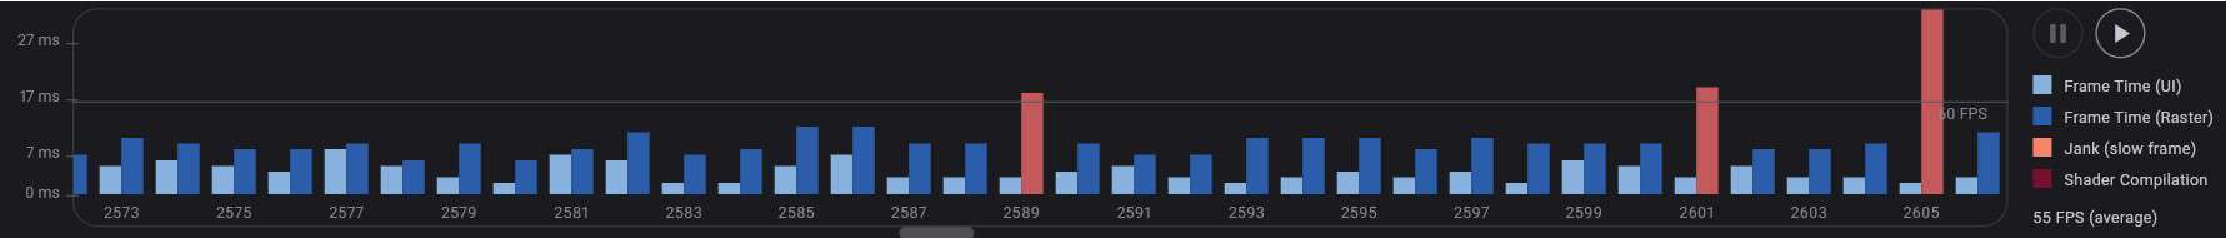
\includegraphics[width=\textwidth]{frontend_performance_graph.pdf}
  \caption{Frontend Render Performance Graph}
  \label{fig:FrontendPerformanceGraph}
\end{figure}

Similarly, NFRT-PR2 focused on general performance on the backend, in particular, response times from the
different endpoints. Various endpoints were accessed about 10 times using Postman and results showed that
backend performance was within expectation for the project. Most of the responses were within 200 ms with the
worst being below 600 ms. The team's expectations for backend performance were for responses to be below 2 seconds
on average according to the SRS, which results from this test show. Below is a graphical representation of the
trials performed and the endpoints tested:

\begin{figure}[H]
  \centering
  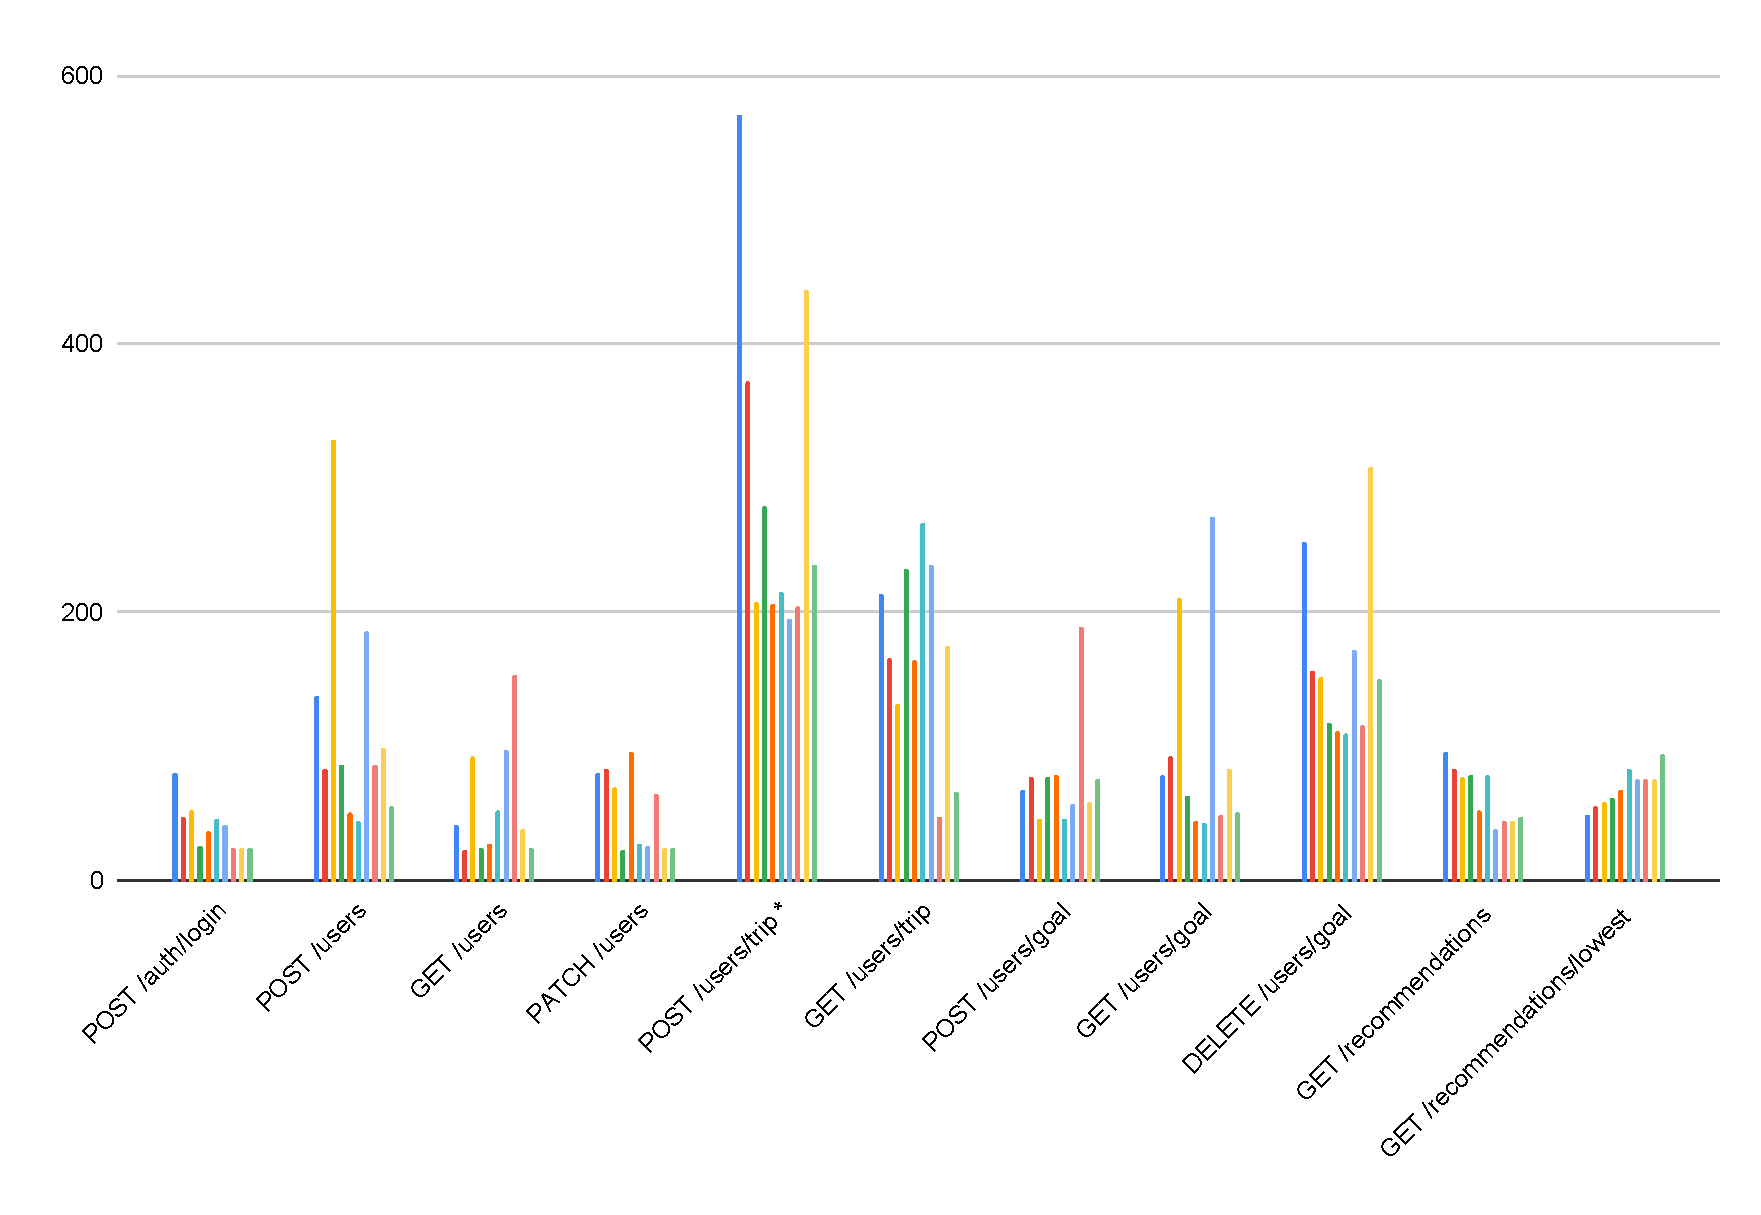
\includegraphics[width=\textwidth]{backend_performance_graph.pdf}
  \caption{Backend Endpoint Performance Graph}
  \label{fig:BacendPerformanceGraph}
\end{figure}

NFRT-PR3 tested the robustness of the backend and involved passing faulty data to see if anything would cause the
system to produce unwanted results. NFRT-PR4 and NFRT-PR5 tested the correctness of the system by verifying how
often users need to correct the OCR and the accuracy of the spending data being returned. Both of these results
were above the expected values, with user correction rate being 5\% and 0.1\% relative error on spending data. Finally,
NFRT-PR6 verifies that the application is within reasonable size, taking up less than 1GB of the user's device
storage. Actual storage consumption was between 300 to 400 MB depending on application usage.

\subsection{Cultural}

This section describes test results for Cultural tests performed as part of the verification
and validation process.

\begin{longtable}{|l|c|}
  \caption{Cultural Testing Summary} \label{Cultural Testing Summary} \\
  \toprule
  \textbf{Test ID} & \textbf{Result} \\
  \midrule
  NFRT-CUR2 & $\checkmark$ \\
  \bottomrule
\end{longtable}

This test was performed internally by team members. NFRT-CUR2 verifies the Classification Engine
and checks that if a new item is submitted into the database, the item's product information can be
properly retrieved.

\subsection{Operation and Environment}

This section describes test results for Operation and Environment tests performed as documented
in the VnV Plan.

\begin{longtable}{|l|c|}
  \caption{Operation and Environment Testing Summary} \label{Operation and Environment Testing Summary} \\
  \toprule
  \textbf{Test ID} & \textbf{Results} \\
  \midrule
  NFRT-OER1 & $\checkmark$ \\
  \midrule
  NFRT-OER2 & $\checkmark$ \\
  \midrule
  NFRT-OER3 & $\checkmark$ \\ 
  \bottomrule
\end{longtable}

These tests were performed internally by team members. NFRT-OER1 verifies the compatibility of the application
on devices using Android 13 or higher. NFRT-OER2 tests that the application interfaces with peripherals properly
such as the device camera. Finally, NFRT-OER3 verifies the CI/CD process and ensures proper unit testing is performed
for updates.

\subsection{Security}

This section covers the test results for Security tests performed as documented in the VnV Plan.

\begin{longtable}{|l|c|}
  \caption{Security Testing Summary} \label{Security Testing Summary} \\
  \toprule
  \textbf{Test ID} & \textbf{Results} \\
  \midrule
  NFRT-SR2 & $\checkmark$ \\
  \bottomrule
\end{longtable}

This test was performed internally by team members. NFRT-SR2 is a test that verifies protections are properly put in
place such that a user cannot modify the database directly (i.e., without using the endpoint).
	
% \section{Comparison to Existing Implementation}	

% This section will not be appropriate for every project.

\section{Unit Testing}

This section will go over the test results from the unit tests made as part of the
verification and validation process.

\subsection{Receipt Extraction Module}

The section provides a brief overview of the unit tests performed and their results for the
Receipt Extraction Module.

\begin{longtable}{|l|c|l|c|l|c|}
  \caption{Receipt Extraction Unit Testing Summary} \label{Receipt Extraction Unit Test Summary} \\
  \toprule
  \textbf{Test ID} & \textbf{Result} & \textbf{Test ID} & \textbf{Result} & \textbf{Test ID} & \textbf{Result} \\
  \midrule
  FRT-M3-1 & $\checkmark$ & FRT-M3-2 & $\checkmark$ & FRT-M3-3 & $\checkmark$ \\
  \midrule
  FRT-M3-4 & $\checkmark$ & FRT-M3-5 & $\checkmark$ & FRT-M3-6 & $\checkmark$ \\
  \midrule
  FRT-M3-7 & $\checkmark$ & FRT-M3-8 & $\checkmark$ & FRT-M3-9 & $\checkmark$ \\
  \midrule
  FRT-M3-10 & $\checkmark$ & FRT-M3-11 & $\checkmark$ & FRT-M3-12 & $\checkmark$ \\
  \midrule
  FRT-M3-13 & $\checkmark$ & FRT-M3-14 & $\checkmark$ & FRT-M3-15 & $\checkmark$ \\
  \midrule
  FRT-M3-16 & $\checkmark$ & FRT-M3-17 & $\checkmark$ & FRT-M3-18 & $\checkmark$ \\
  \midrule
  FRT-M3-19 & $\checkmark$ & FRT-M3-20 & $\checkmark$ & FRT-M3-21 & $\checkmark$ \\
  \midrule
  FRT-M3-22 & $\checkmark$ & FRT-M3-23 & $\checkmark$ & FRT-M3-24 & $\checkmark$ \\
  \midrule
  FRT-M3-25 & $\checkmark$ & FRT-M3-26 & $\checkmark$ & ~ & ~ \\
  \bottomrule
\end{longtable}

To summarize, tests FRT-M3-1 to FRT-M3-26 are all frontend tests. These tests focus on the helper functions used
to extract specific information when receiving a chunk of receipt text. FRT-M3-1 to FRT-M3-6 focus on date
extraction with different formats, FRT-M3-7 to FRT-M3-13 test address extraction, FRT-M3-14 to FRT-M3-16 target grocery item extraction,
FRT-M3-17 to FRT-M3-19 focus on subtotal cost extraction, and FRT-M3-20 to FRT-M3-22 tests total cost extraction.
Finally, FRT-M3-23 to FRT-M3-24 and FRT-M3-25 to FRT-M3-26 test updating and JSON conversion for the Item and Grocery Trip
objects respectively. In general, these
tests consist of ideal use cases as well as some edge cases that may appear during use.
For more detailed information regarding the Receipt Extraction Module unit tests, the testing file
can be found here: \href{https://github.com/allanfang1/grocery_spending_tracker_app/blob/main/test/receipt_extraction_test.dart}{receipt extraction
unit tests}.

\subsection{User Analytics Module}

...

\subsection{Users Module}

...

\subsection{Authentication Module}

...

\subsection{Recommendation Engine}

...

\subsection{Classification Engine}

...

\section{Changes Due to Testing}

% \wss{This section should highlight how feedback from the users and from 
% the supervisor (when one exists) shaped the final product.  In particular 
% the feedback from the Rev 0 demo to the supervisor (or to potential users) 
% should be highlighted.}

Prior to formal usability testing, user impressions of the Revision 0 version of the app
generally criticized the usability of the application. Specifically, better communication with
the user in terms of loading. The previous version of the application lacked animated loading
indicators so for forms that had a server request attached to them, they believed the application
to be frozen after submission. This resulted in cases where users would try submitting again producing
a duplicate server request. This has since been resolved by adding various animated loading indicators
and overlays to prevent double clicking a submission and better communicate to users when server requests
were being processed. Some intuitiveness features were also added as a result of user feedback such as
tap focus on the receipt capture page. Additionally, some feedback received from the Revision 0 demo
was addressed in the current version of the application. This included more detailed information
on the Goals page and matching address to a list of known addresses to improve usability/reduce user
input.\\

During formal usability testing of the current application version, much of the feedback had to do with robustness
of the application as opposed to functionality. In particular, the request for submitting a trip
in some cases ended up taking close to 10 seconds due to the current Classification Engine implementation. As
a result, users believed that there was something wrong with the application or that there was an error. In response to this,
a backend fix is being worked on to reduce the response time which will be done prior to Revision 1.
Additionally, some users had some issues with the receipt capture, not knowing that they had to get the
receipt to occupy as much of the camera frame as possible for the best results, so an information screen
on this page is being worked on to better help users with receipt capture which will also be finished
prior to Revision 1. Outside of the UI/UX, users found that recommendations could be improved more
in terms of accuracy relating to the user's purchase history which the team will try to do before Revision 1
as well.

\section{Automated Testing}

On the frontend, all automated tests are carried out using Flutter's built-in testing package.
All tests are located in the "test" folder which is organized by components being tested (found 
\href{https://github.com/allanfang1/grocery_spending_tracker_app/tree/main}{here}). For example,
the \textit{profile\_provider\_test} file executes tests related to the provider for profile functionality.
These tests are executed twice during the development workflow: the first is locally while working on
individual feature branches and the second is on merges/pushes to the "dev" branch of the frontend repository.
The first execution is done manually using \textit{flutter test} in the command line and the second is done
automatically using \textit{Github Actions}.\\

On the backend, automated tests are done using Chai HTTP. Tests are located in the "tests" folder which
is then organized by component and the module being tested 
(found \href{https://github.com/grocery-spending-tracker/grocery-spending-tracker-backend/tree/master/tests}{here}).
As an example, the \textit{userController.analytics.test} file contains unit tests related to the Analytics Module
functionality in the user controller.
These tests are automatically executed during the deployment process of the backend when code is pushed to the
"master" branch of the backend repository. This process is handled by \textit{Github Actions}.
		
\section{Trace to Requirements}
		
\section{Trace to Modules}		

\section{Code Coverage Metrics}

\bibliographystyle{plainnat}
\bibliography{../../refs/References}

\newpage{}
\section{Appendix --- Survey Results}

\subsection{Functional Requirement Survey Questions}
\subsubsection{Survey questions for \textbf{FRT-FR1-2}.}

\begin{enumerate}
\item How easy was it to log into the application?
Responses: \{(not easy) 1, 2, 3, 4, 5 (very easy)\} \\
  \begin{itemize}
    \item On average, a 5. The login process was as expected for users.
  \end{itemize}
\end{enumerate}

\subsubsection{Survey questions for \textbf{FRT-FR8-2}.}

\begin{enumerate}
  \item How useful would you say that the application recommendations are to you?
  Responses: \{(not useful) 1, 2, 3, 4, 5 (very useful)\} \\
    \begin{itemize}
      \item On average, a 3.5. Some recommendations were not 100\% accurate for the user but about at the
      expected value for fit criterion.
    \end{itemize}
  \item How likely are you to act the recommendation provided to you by the application?
  Responses: \{(not likely) 1, 2, 3, 4, 5 (very likely)\}
    \begin{itemize}
      \item On average, a 3. Users would need to see some more accuracy improvements before acting on a recommendation.
    \end{itemize}
\end{enumerate}

\subsection{Look and Feel Survey Questions}

\begin{enumerate}
  \item Did you feel the colour scheme was cohesive and consistent throughout the application?
    \begin{itemize}
      \item General consensus was that colour scheme consistency and cohesiveness was not an issue.
      \item General theme had purples and whites, which was consistent overall.
    \end{itemize}
  \item On a scale of 1-10, how would you rate the general layouts of each of the pages?
    \begin{itemize}
      \item On average, an 8. Users found the layouts easy to understand and navigate.
      \item Pages were not found to be too overwhelming in terms of features.
      \item Layouts/components on the page could be more creative.
      \item Similar to existing applications such as Instagram.
    \end{itemize}
  \item Did the general layouts of the application pages appear consistent throughout navigation?
    \begin{itemize}
      \item The consensus was that layouts were pretty consistent across the different pages.
      \item Layouts were similar enough where users were generally able to figure out the different
      features on the pages without issue.
    \end{itemize}
  \item On a scale of 1-10, how would you rate how features were organized?
    \begin{itemize}
      \item On average, a 9. All features were where users expected them.
      \item Features generally fit the main idea of the pages that they were present on.
    \end{itemize}
  \item Were there any places where you expected loading indicators but there weren't any or vice versa?
    \begin{itemize}
      \item Loading indicators/communication was well received for this version of the application.
      \item Many of the users who had seen the previous version of the application with less loading screens
      said the application was much improved in that aspect.
      \item Users felt that the application properly communicated when processes were occurring throughout
      the application.
      \item With general usage, users found that application never felt "frozen" or "stuck".
    \end{itemize}
  \item Do you have any feedback on the overall look and feel of the application?
    \begin{itemize}
      \item In terms of how functional the appearance of the application was, there were no complaints.
      \item Some users voiced that in terms of visual appeal, the application was lacking (i.e. boring/lacking
      in creativity compared to other apps).
      \item Application is very minimal so some minor decorations could help make app more engaging, but generally
      a minor complaint.
    \end{itemize}
\end{enumerate}

\subsection{Usability Survey Questions}

\begin{enumerate}
  \item What parts of the application were easiest for you to understand/learn?
    \begin{itemize}
      \item Receipt confirmation form was easy for users to fill out for the first time
      \item History page was also very easy for users to use and understand
      \item Goals page took users slightly longer than the other pages but were able to figure features
      out without intervention and in reasonable time
    \end{itemize}
  \item What parts of the application do you feel additional explanation or clarity could be provided?
    \begin{itemize}
      \item The receipt capture functionality could use some more clarification as it is not intuitively
      clear that filling the receipt in the camera frame produces the best results
    \end{itemize}
  \item Was the language and wording used in the application understandable and inoffensive? If not, please
  provide where and how the wording could be improved?
    \begin{itemize}
      \item Language was generally understood and nothing was offensive to the users.
    \end{itemize}
  \item Were there any issues you encountered while using the application?
    \begin{itemize}
      \item For some users, the submission of their grocery trip took a very long time, close to 10 seconds.
      This caused them to believe something was wrong with the application due to the length of time it was processing
      for.
    \end{itemize}
  \item Did you have any issues with navigating the application? If you made a mistake, were you able to navigate
  back to where you started?
    \begin{itemize}
      \item No issues with navigation. Navigation bar was very responsive and navigating back to previous
      pages was always available.
      \item Users liked how navigation was always available making it easy to find their way back to where
      they started.
    \end{itemize}
  \item On a scale of 1-10, how would you rate the usability and intuitiveness of the application?
    \begin{itemize}
      \item On average, the score was an 8. Besides the hiccups with receipt submission and better communication
      for how the receipt should be captured, users found the app to be easy to navigate.
      \item Navigation and layouts were similar to other apps they had used so learning curve was not
      too difficult.
      \item Very little intervention from members of the team was needed to help users.
    \end{itemize}
\end{enumerate}

\newpage{}
\section*{Appendix --- Reflection}

The information in this section will be used to evaluate the team members on the
graduate attribute of Reflection.  Please answer the following question:

\begin{enumerate}
  \item In what ways was the Verification and Validation (VnV) Plan different
  from the activities that were actually conducted for VnV?  If there were
  differences, what changes required the modification in the plan?  Why did
  these changes occur?  Would you be able to anticipate these changes in future
  projects?  If there weren't any differences, how was your team able to clearly
  predict a feasible amount of effort and the right tasks needed to build the
  evidence that demonstrates the required quality?  (It is expected that most
  teams will have had to deviate from their original VnV Plan.)
\end{enumerate}

During the testing process, we found that the scope of our actual
implementation had changed somewhat compared to what we had planned the application to be
initially. Given the VnV Plan was written prior to any implementation, we did not have
the clearest vision of what the project was going to be. One big example of this was
with the Recommendation Engine and User Goals. When writing the VnV Plan, we had imagined them
to be more coupled such that we could have recommendations that would specifically help users
stay within goals and goals would be available for specific products. The actual implementation
we ended up creating ended up being more general, where User Goals are more related to overall
spending and recommendations currently exclusively consider a user's purchase history.
Similar scope/requirement changes appeared in other parts of the development process resulting in
various changes overall being made to the VnV Plan such that it aligned better with our implementation.\\

In order to better anticipate this kind of change in future projects, we believe that better planning
would be needed. The reason these changes had to be made was because we had not fully realized our ideas
for the project. Additionally, as development occurred, we realized certain aspects of the application
were less feasible than we thought given our development period and knowledge of the technology. If more research
and planning had been done prior to the creation of the VnV Plan, it is possible that the tests would have been closer
to our current product. In conclusion, changes to the VnV Plan had to be made due to scope changes throughout
development. These changes could be better anticipated if more research and planning had been done at
an earlier point.
\end{document}